To evaluate the network, we use a fixed evaluation set consisting of interactions for the three nuclei \n{2}{H}, \n{3}{H} and \n{4}{He}, which were also used in the training as well as the nucleus \n{6}{Li}, to test the extrapolation on a nucleus which was previously unseen by the network. For evaluation, we use semilocal momentum space regulated chiral interactions. Furthermore, each interaction will get evaluated using an SRG evolved hamiltonian with flow parameters of $\eta = \SI{0.04}{\femto\metre^4}$ and $\eta = \SI{0.08}{\femto\metre^4}$, to analyze the extrapolations in dependence on the flow parameter. These interactions belong to a different family than the interactions used in training. This means that the network still has to perform an extrapolation, even for the reused nuclei \n{2}{H}, \n{3}{H} and \n{4}{He}.

\begin{wrapfigure}{r}{.5\textwidth}
  \centering
  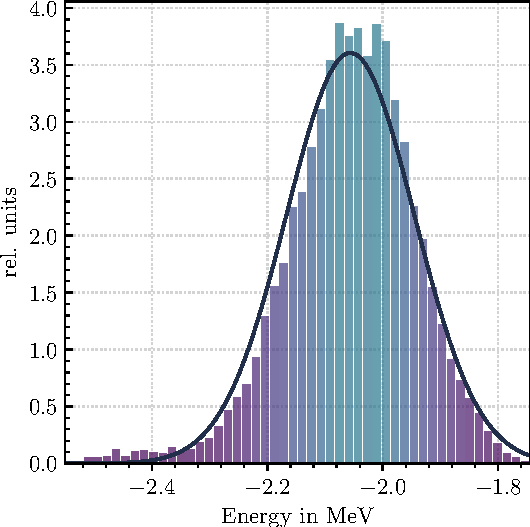
\includegraphics[width=.5\textwidth]{media/example_histogram.pdf}
  \caption{An example normed histogram of evaluations for the \textit{chi2bSMSI2B} interaction of \n{2}{H} using a SRG flow parmeter of \srg{0.04}. The networks are evaluated using sequences from $N_\mathrm{max}=6$ to $N_\mathrm{max}=12$}.
  \label{fig:example_histogram}
\end{wrapfigure}
In the previous section we described the training process of a single network. Since one network can only output one prediction for a given input sequence, we cannot generate a big enough evaluation statistic if we only evaluate the data with one network. To fix that, we train multiple networks which will be evaluated. For our work, we train 100 networks to generate a broad statistic.


Since the networks should be applied to heavier nuclei, for which NCSM calculations cannot be done for sufficiently large $N_\mathrm{max}$, we want to analyze how the evaluation changes if we restrict the evaluation samples to certain $N_\mathrm{max}$ values. We want to demonstrate this evaluation process using the example of the \textit{chi2bSMSI2B} interaction of \n{2}{H} with a SRG flow paramter of \srg{0.04}, for which NCSM calculations have been done with 7 frequencies from $\hbar\Omega = \SI{16}{\mega\electronvolt}$ to $\hbar\Omega = \SI{40}{\mega\electronvolt}$. To simulate a real use case of extrapolation, we first want to restrict the evaluation process to sequences with $N_\mathrm{max}$ values of 6, 8, 10, 12. Since there are more than 3 frequencies available, a similar inflation process as described in the previous section will format the sequences according to the network structure. Now, every single sample can be evaluated by every of the 100 trained networks to get a broad histogram of predictions. A sample histogram can be seen in \autoref{fig:example_histogram}.


To quantify the evaluation of the networks, we can calculate the mean evaluation as the extrapolated ground state energy as well as the standard deviation to express the error of the extrapolation. To see how the evaluation changes if we consider sequences of higher $N_\mathrm{max}$, we also do this evaluation process for sequences with maximum $N_\mathrm{max}$ of 16, 20 and 24. The data for all those evaluations will be condensed in a single plot for a given nucleus and interaction. In \autoref{fig:example_evaluation}, we see the evaluation of the example interaction from above.

\begin{figure}[H]
  \centering
  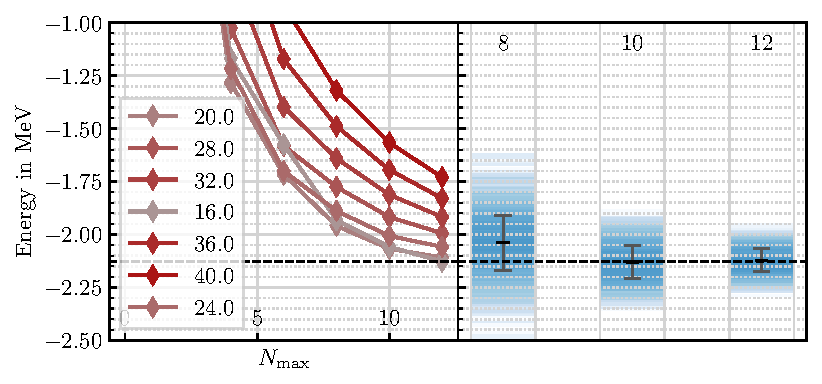
\includegraphics[]{media/example_evaluation.pdf}
  \caption{An example histogram of evaluations for the \textit{chi2bSMSI2B} interaction of \n{2}{H} using a SRG flow parmeter of \srg{0.04}. On the left side the raw NCSM calculations are shown to compare them to the extrapolation. On the right side, for each maximum $N_\mathrm{max}$, the histogramm as well as its mean and standard deviation is shown, which represent the extrapolated energy and its uncertainty.}
  \label{fig:example_evaluation}
\end{figure}
